%!TEX root = ../main.tex
\chapter{Timing: Additional Plots}
\label{appendix:TimingAdd}

\begin{figure}[htbp!]
  \centering
  \begin{subfigure}[t]{0.5\textwidth}
    \centering
    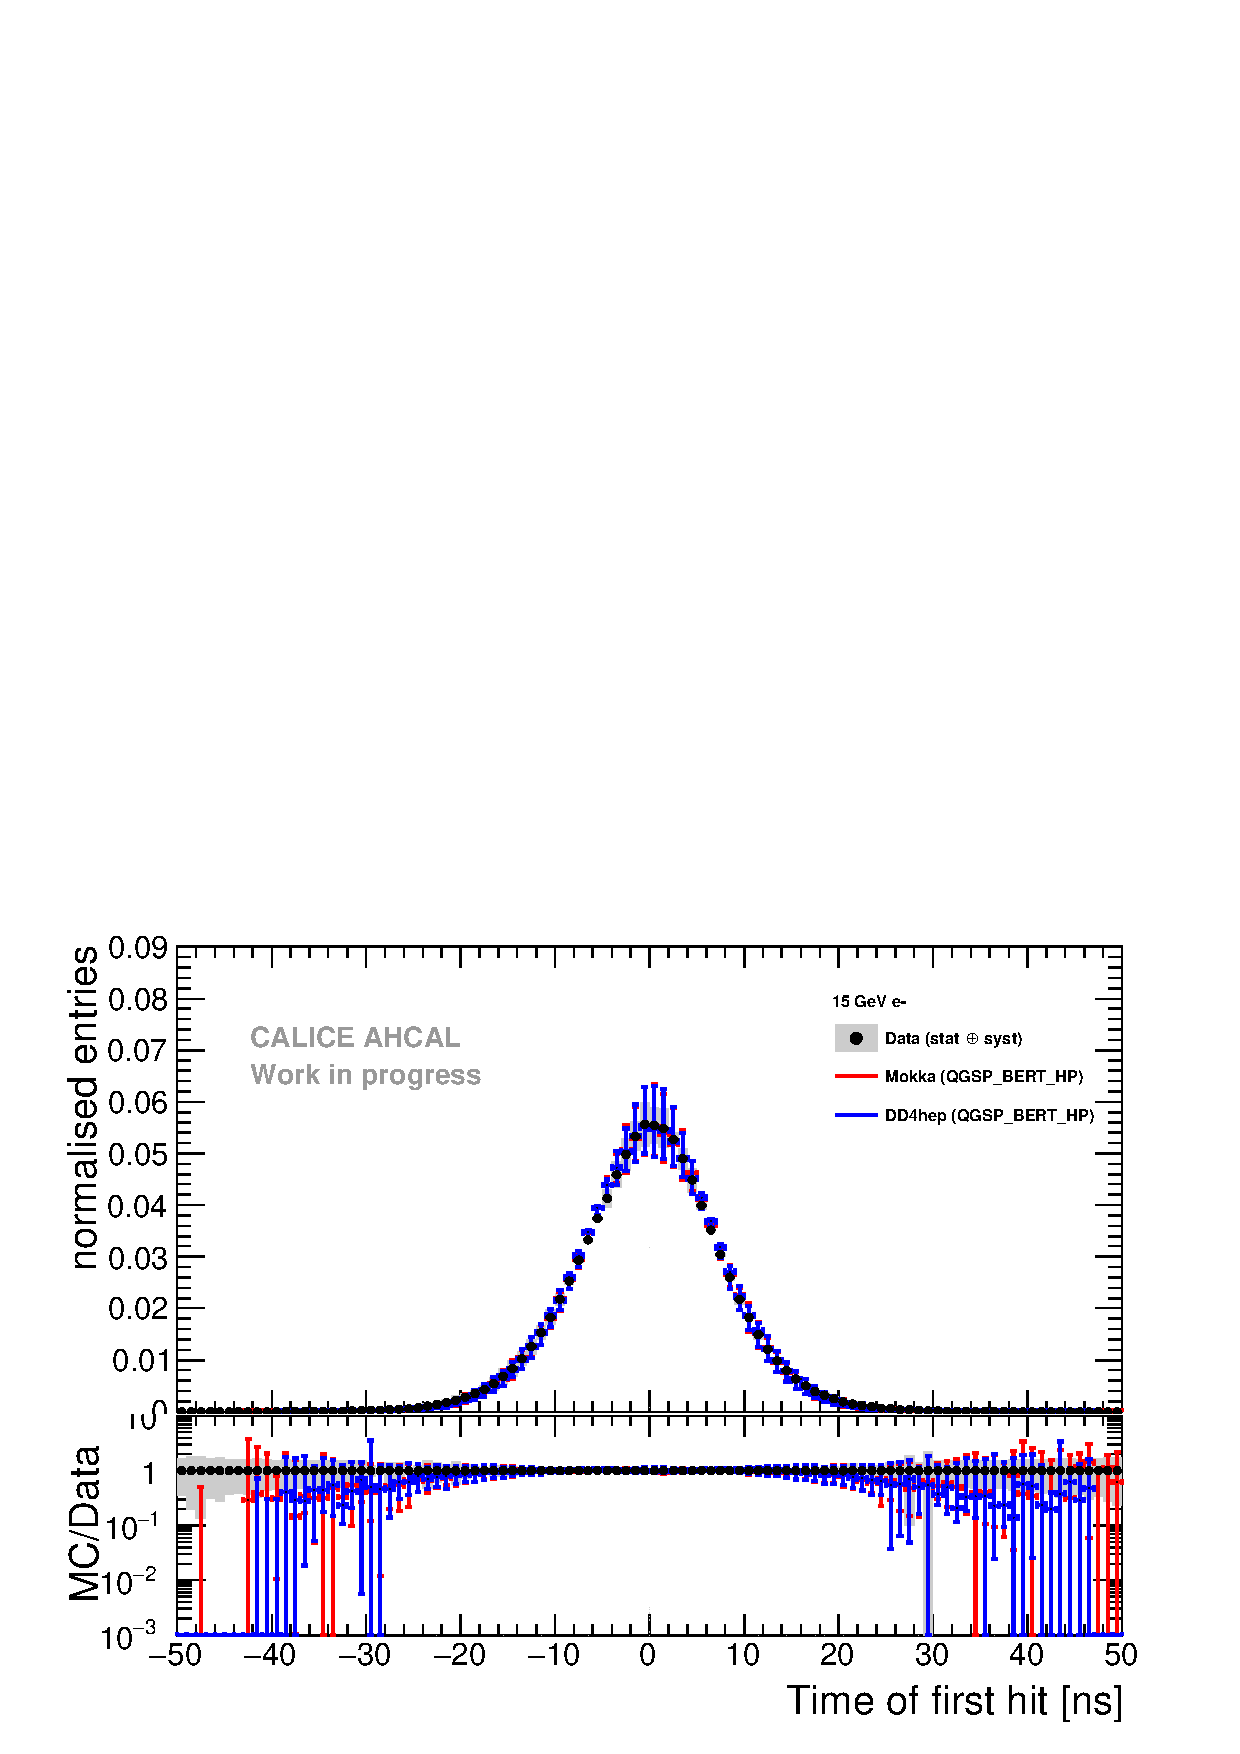
\includegraphics[width=1\textwidth]{../Thesis_Plots/Timing/Electrons/Plots/Comparison_SimData_Electrons15GeV.pdf}
    \caption{15 GeV.}\label{fig:elec_sim_data_15GeV}
  \end{subfigure}
  \hfill
  \begin{subfigure}[t]{0.5\textwidth}
    \centering
    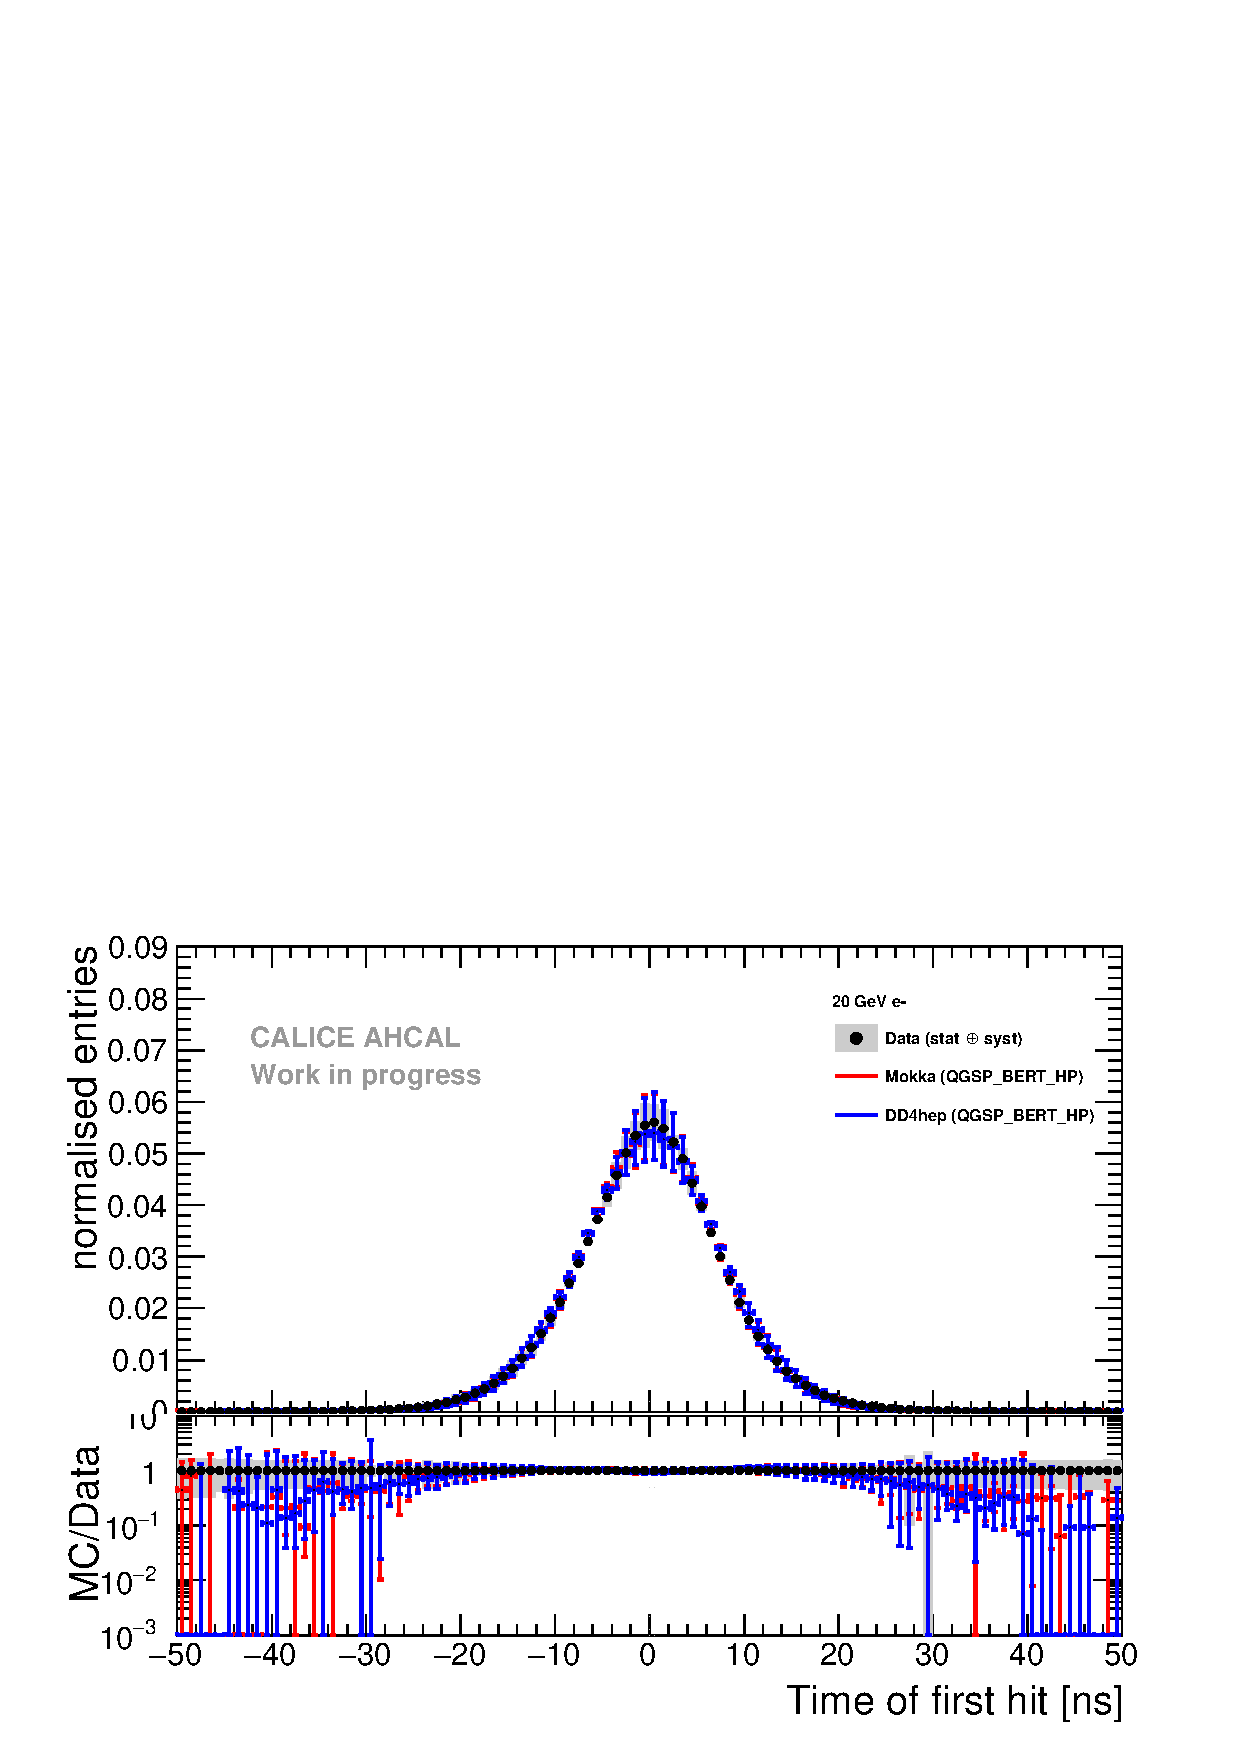
\includegraphics[width=1\textwidth]{../Thesis_Plots/Timing/Electrons/Plots/Comparison_SimData_Electrons20GeV.pdf}
    \caption{20 GeV.}\label{fig:elec_sim_data_20GeV}
  \end{subfigure}
  \hfill
  \begin{subfigure}[t]{0.5\textwidth}
    \centering
    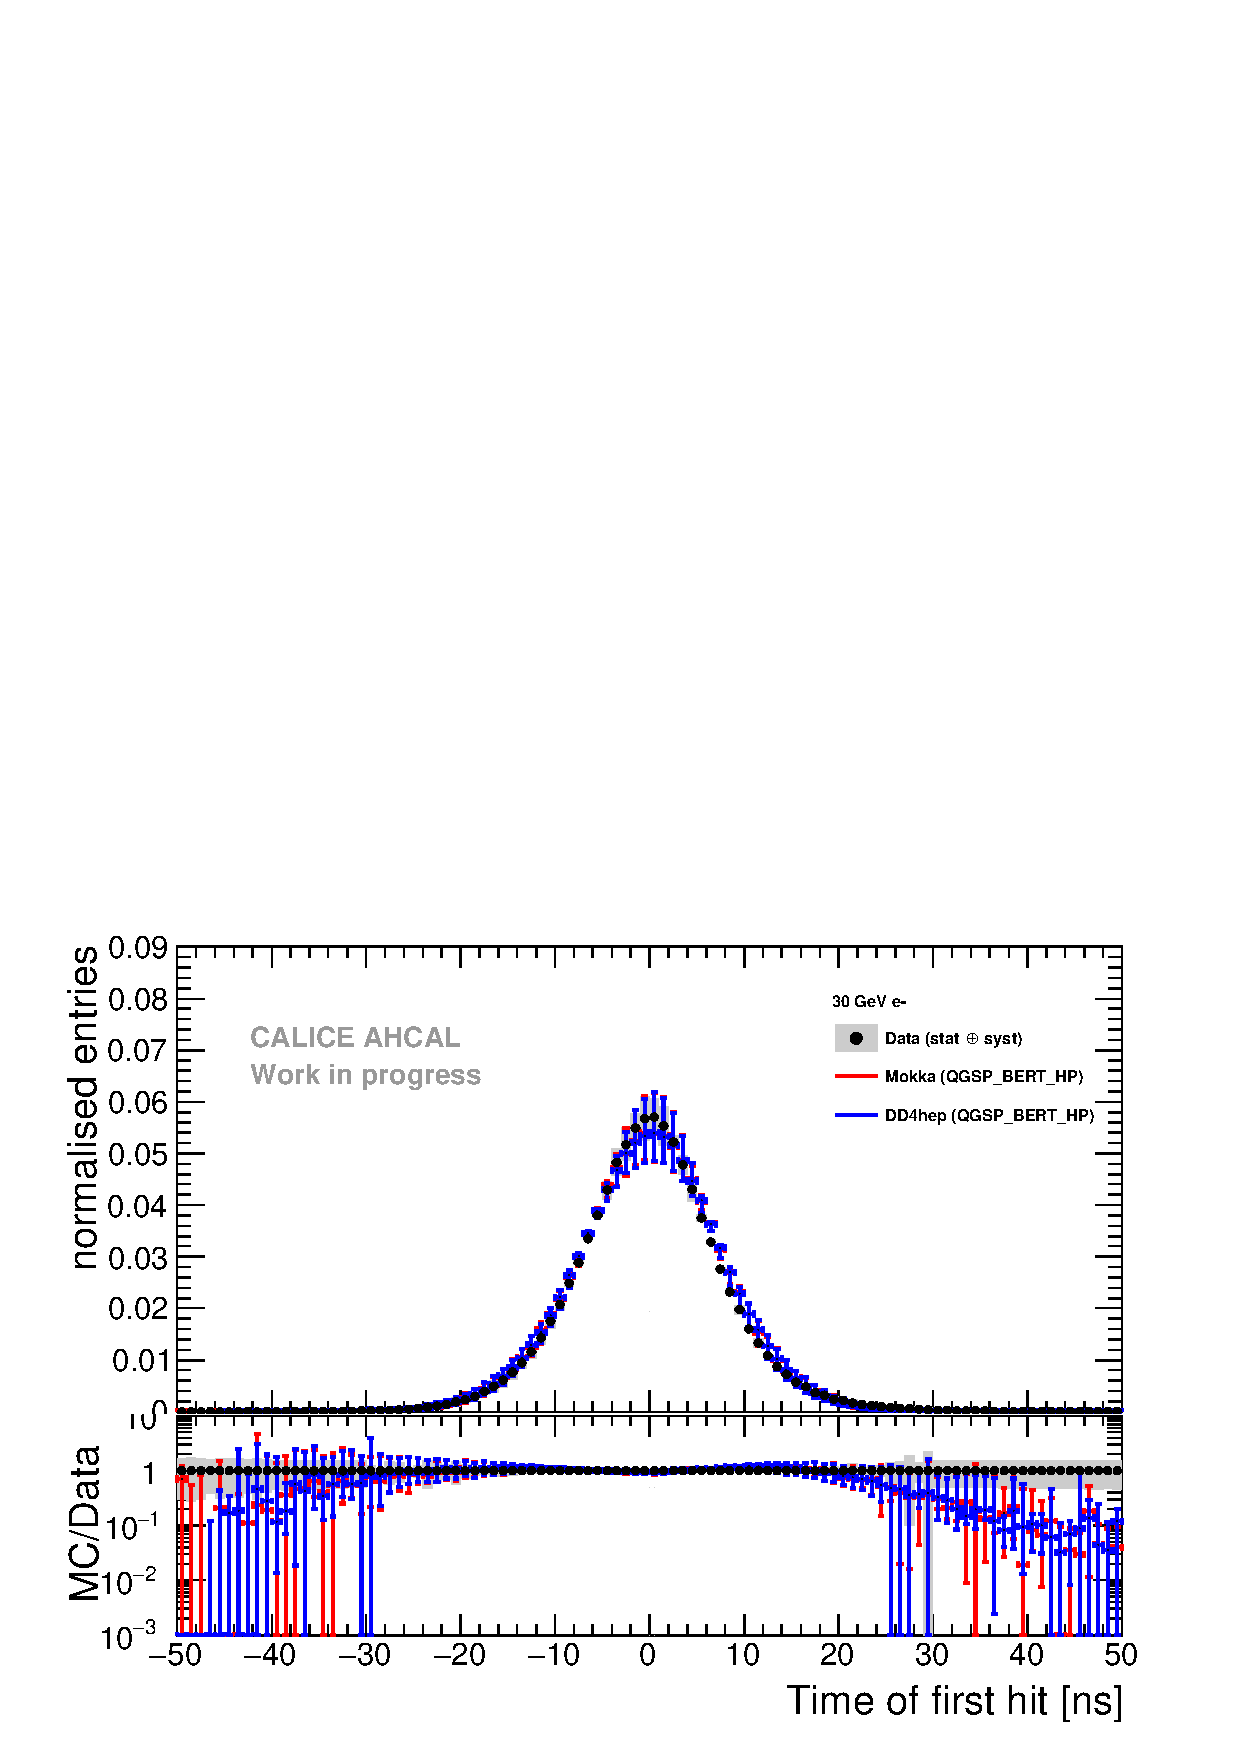
\includegraphics[width=1\textwidth]{../Thesis_Plots/Timing/Electrons/Plots/Comparison_SimData_Electrons30GeV.pdf}
    \caption{30 GeV.}\label{fig:elec_sim_data_30GeV}
  \end{subfigure}
  \hfill
  \begin{subfigure}[t]{0.5\textwidth}
    \centering
    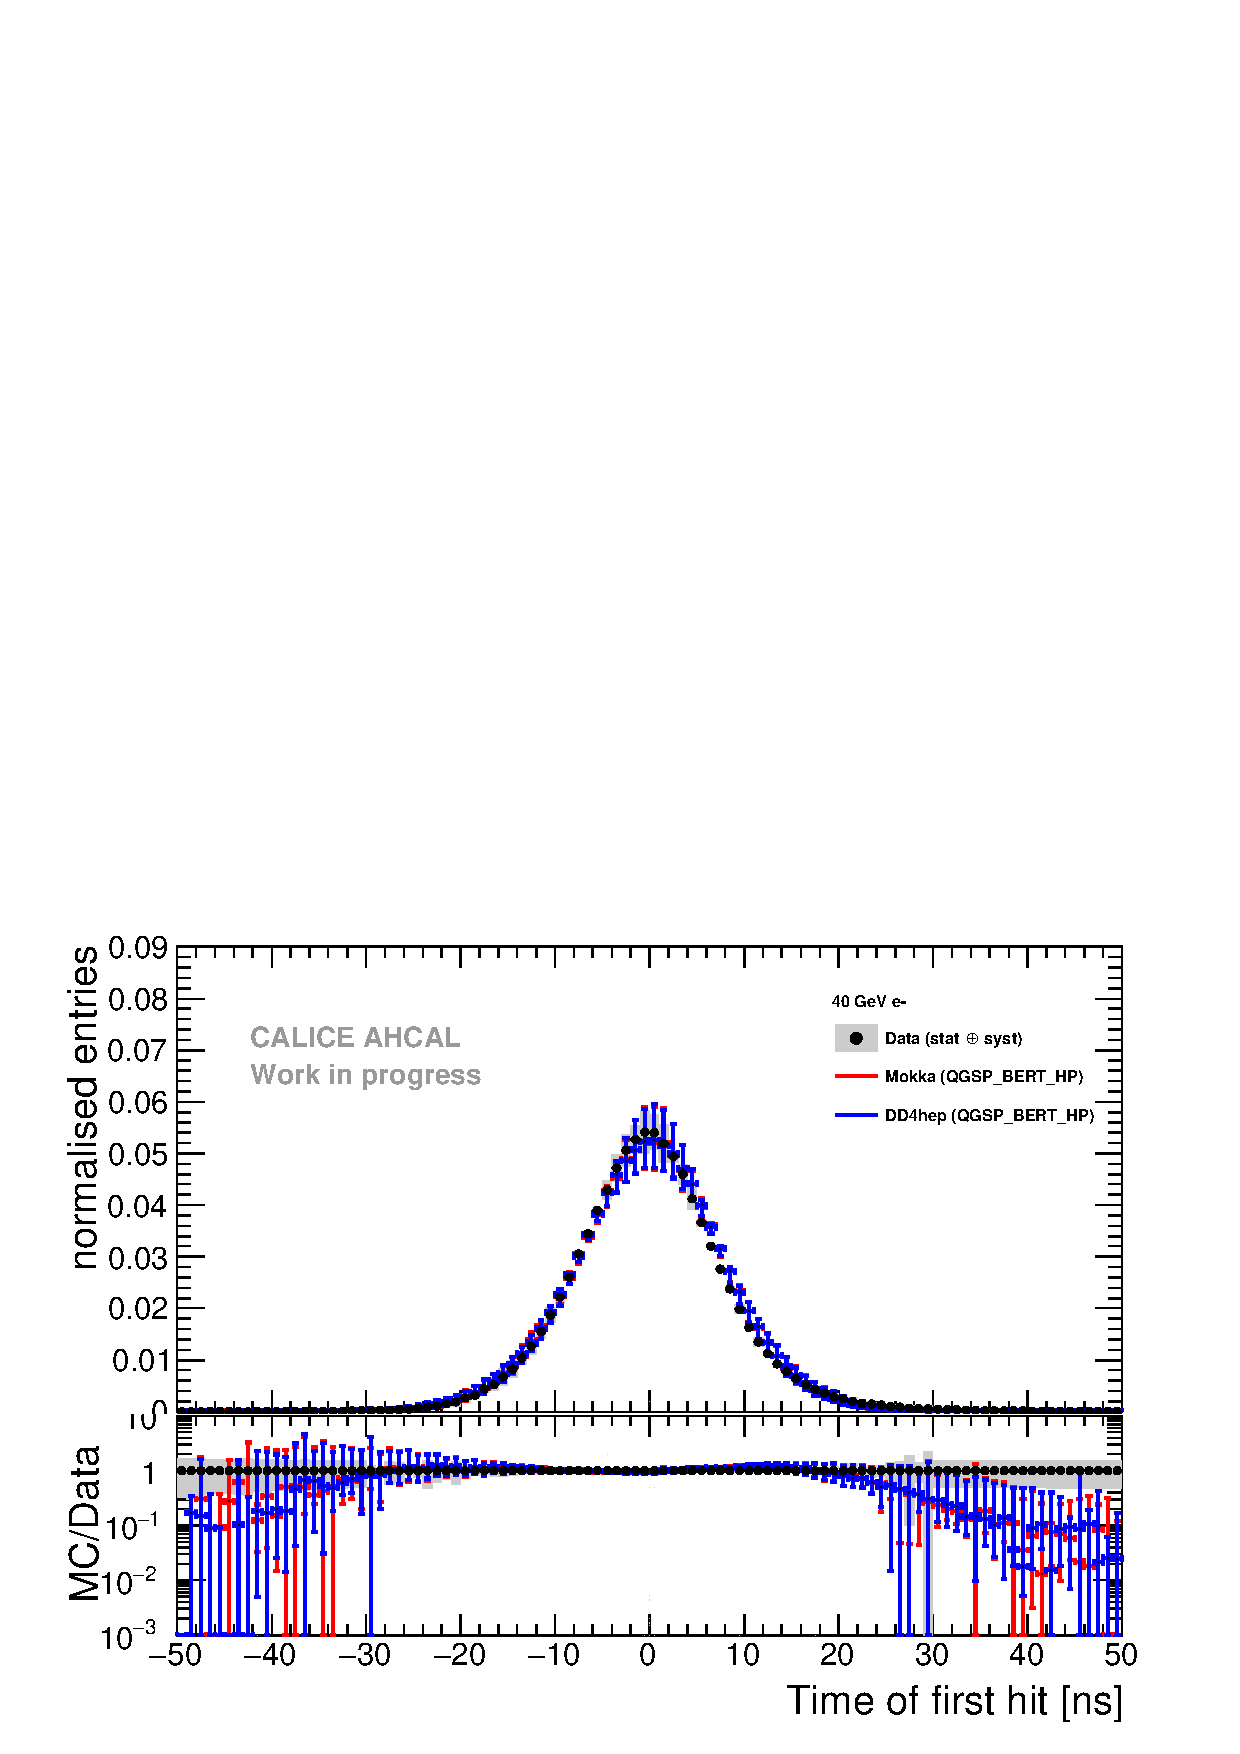
\includegraphics[width=1\textwidth]{../Thesis_Plots/Timing/Electrons/Plots/Comparison_SimData_Electrons40GeV.pdf}
    \caption{40 GeV.}\label{fig:elec_sim_data_40GeV}
  \end{subfigure}
  \hfill
  \begin{subfigure}[t]{0.5\textwidth}
    \centering
    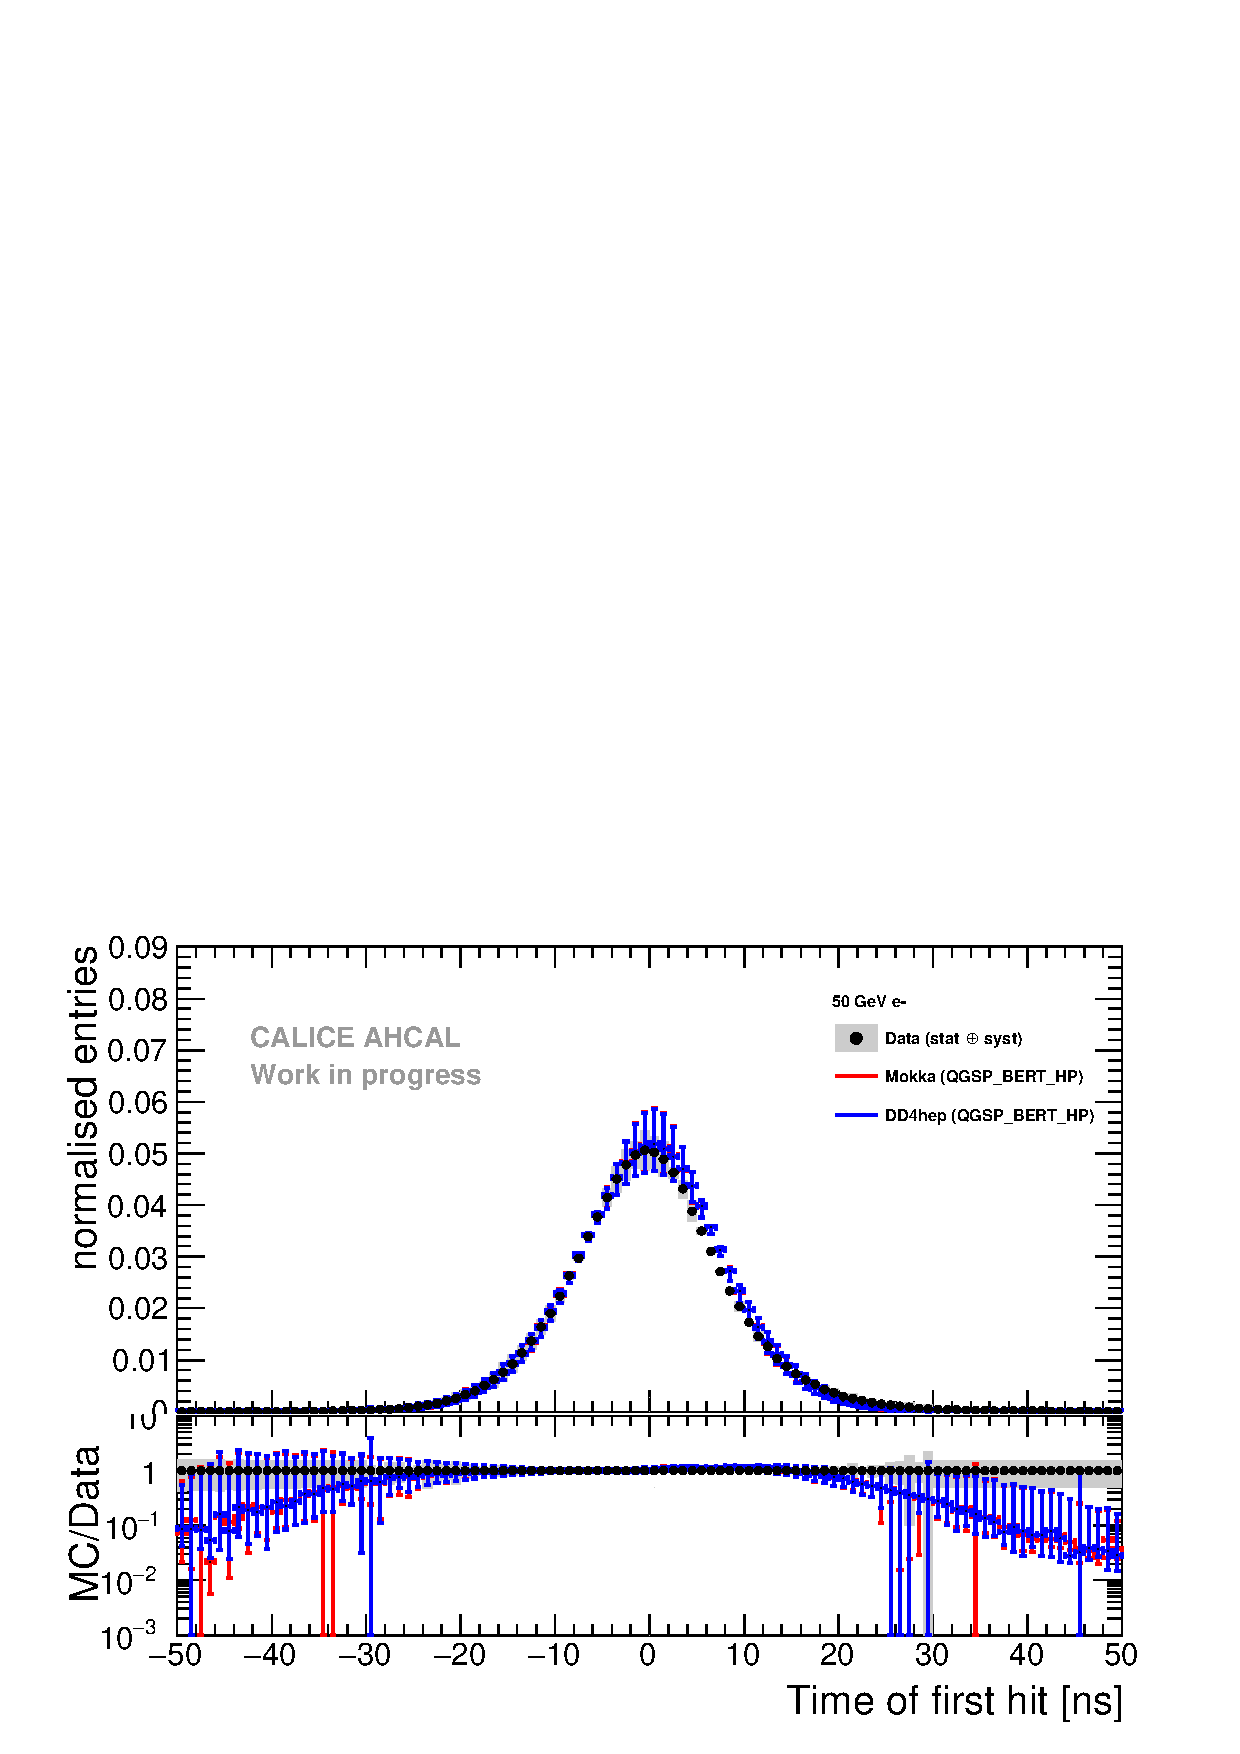
\includegraphics[width=1\textwidth]{../Thesis_Plots/Timing/Electrons/Plots/Comparison_SimData_Electrons50GeV.pdf}
    \caption{50 GeV.}\label{fig:elec_sim_data_50GeV}
  \end{subfigure}
  \caption{Comparison between electron data and MC for all energies of the time of first hit. The grey area represents the statistical and systematical error of the data. Error bars in simulation are obtained by varying the cross-talk parameter and with the error envelope from the number of hits parametrization.} \label{fig:sim_data_elec_add}
\end{figure}

\begin{figure}[htbp!]
  \begin{subfigure}[t]{0.5\textwidth}
    \centering
    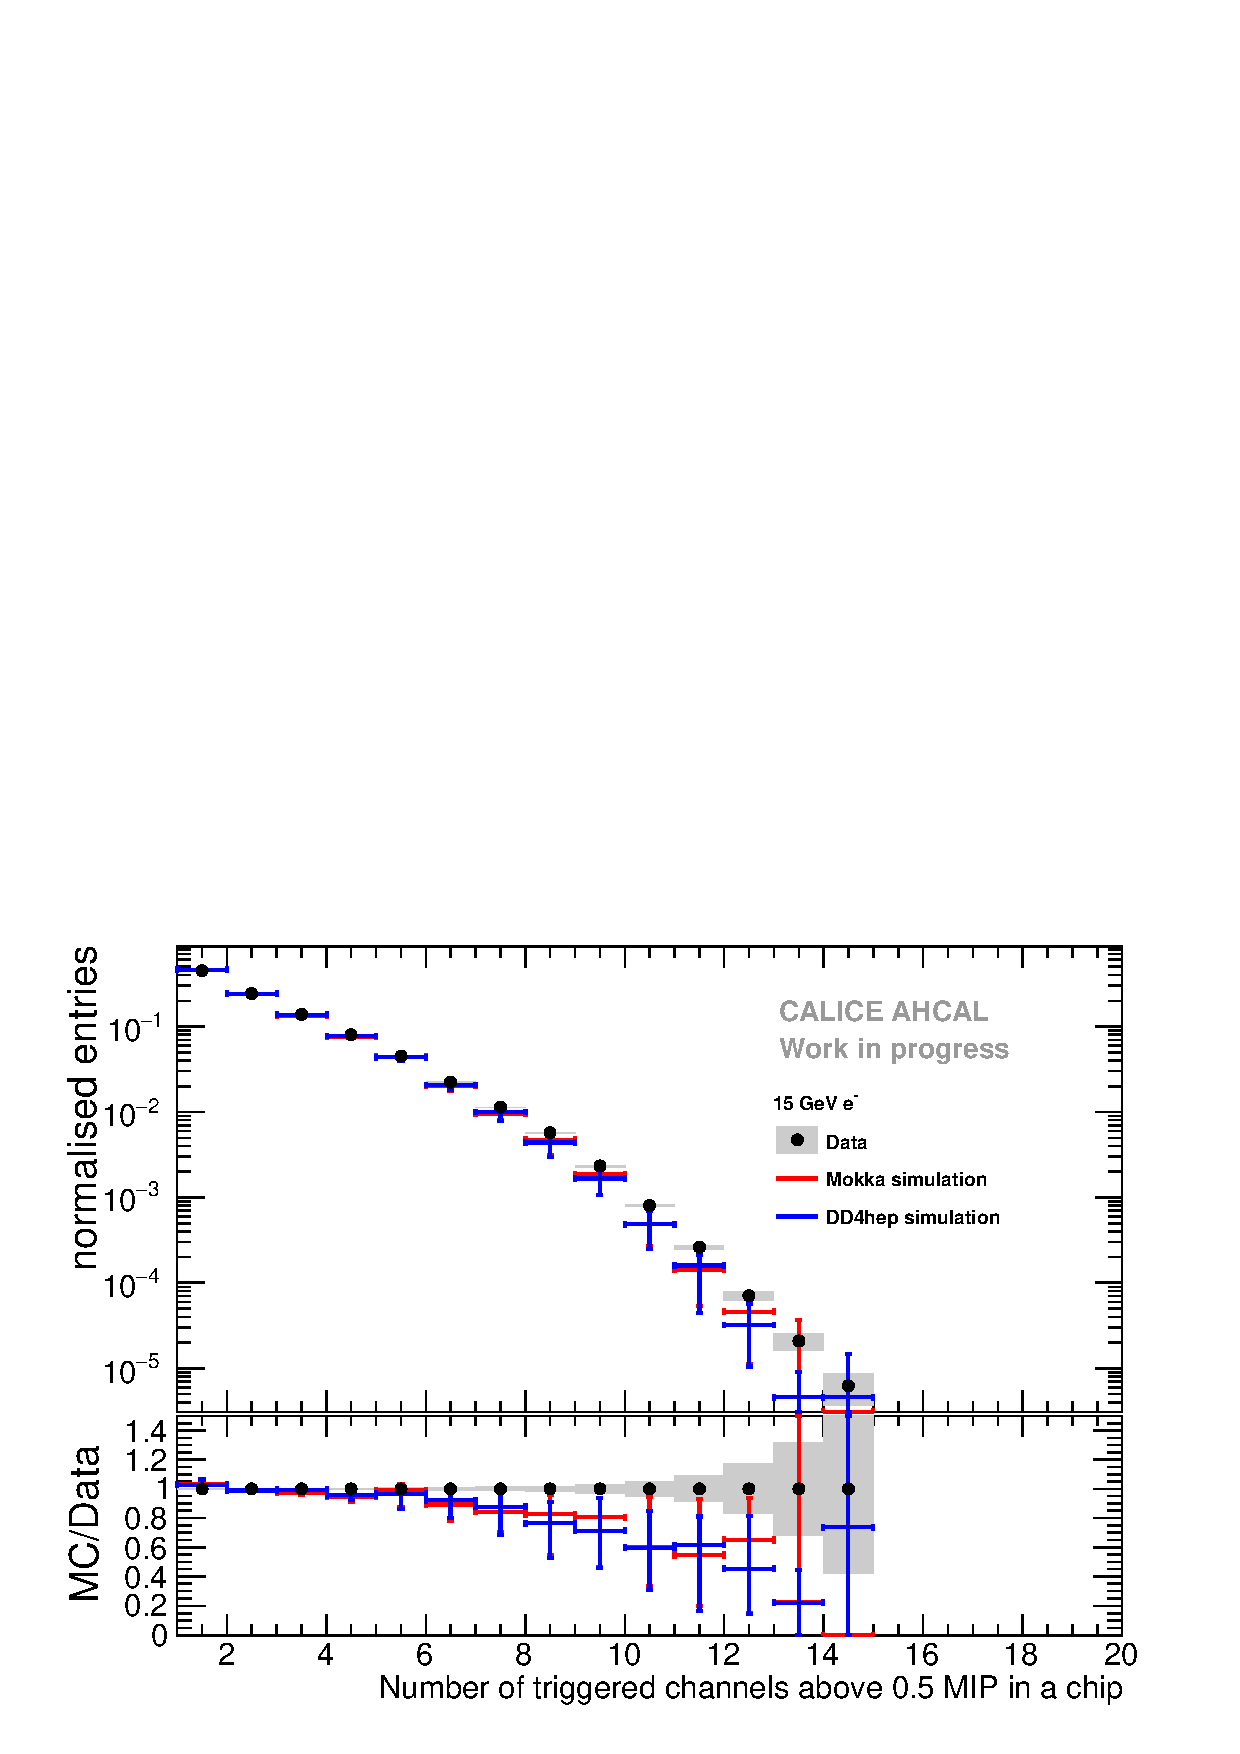
\includegraphics[width=1\textwidth]{../Thesis_Plots/Timing/Electrons/Plots/Comparison_SimData_Electrons_nHits_15GeV.pdf}
    \caption{15 GeV.}\label{fig:elec_sim_data_nHits_15GeV}
  \end{subfigure}
  \hfill
  \begin{subfigure}[t]{0.5\textwidth}
    \centering
    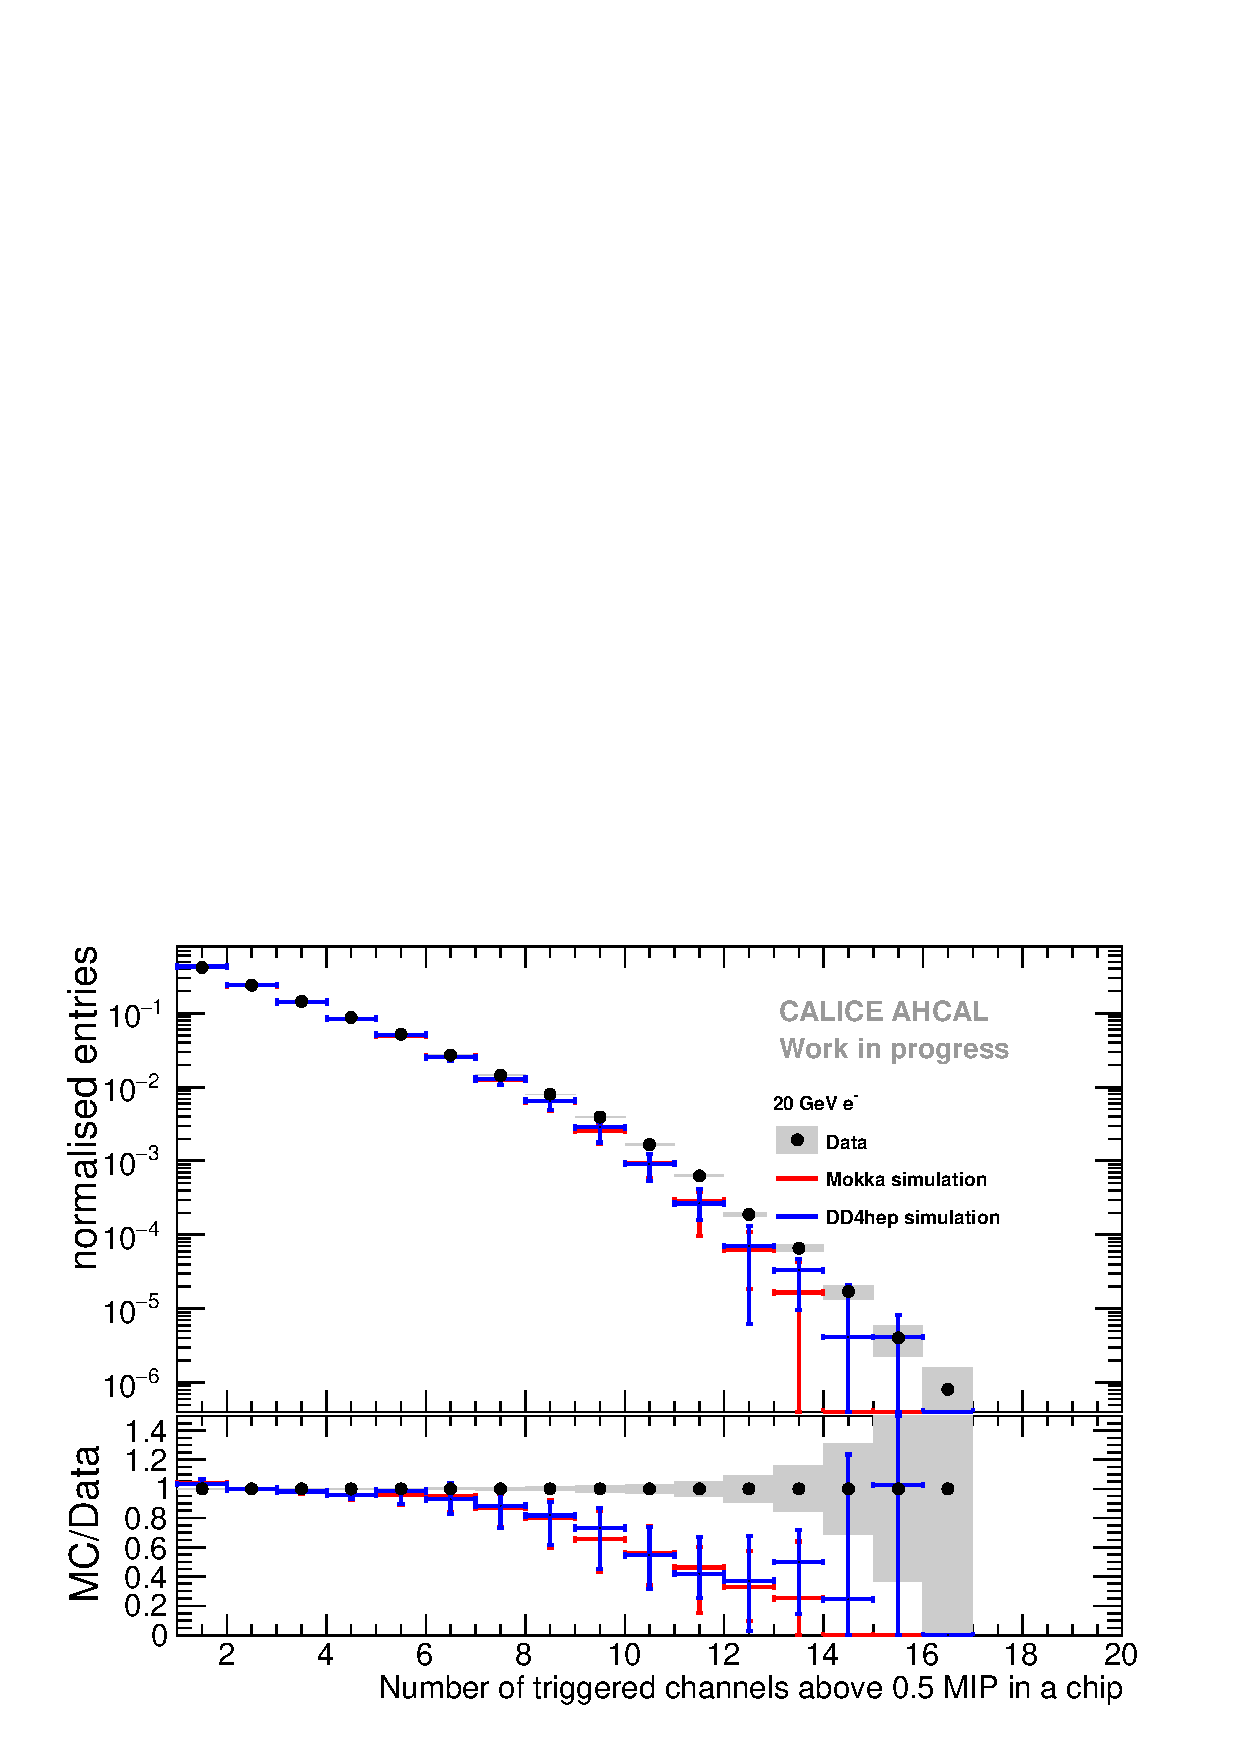
\includegraphics[width=1\textwidth]{../Thesis_Plots/Timing/Electrons/Plots/Comparison_SimData_Electrons_nHits_20GeV.pdf}
    \caption{20 GeV.}\label{fig:elec_sim_data_nHits_20GeV}
  \end{subfigure}
  \hfill
  \begin{subfigure}[t]{0.5\textwidth}
    \centering
    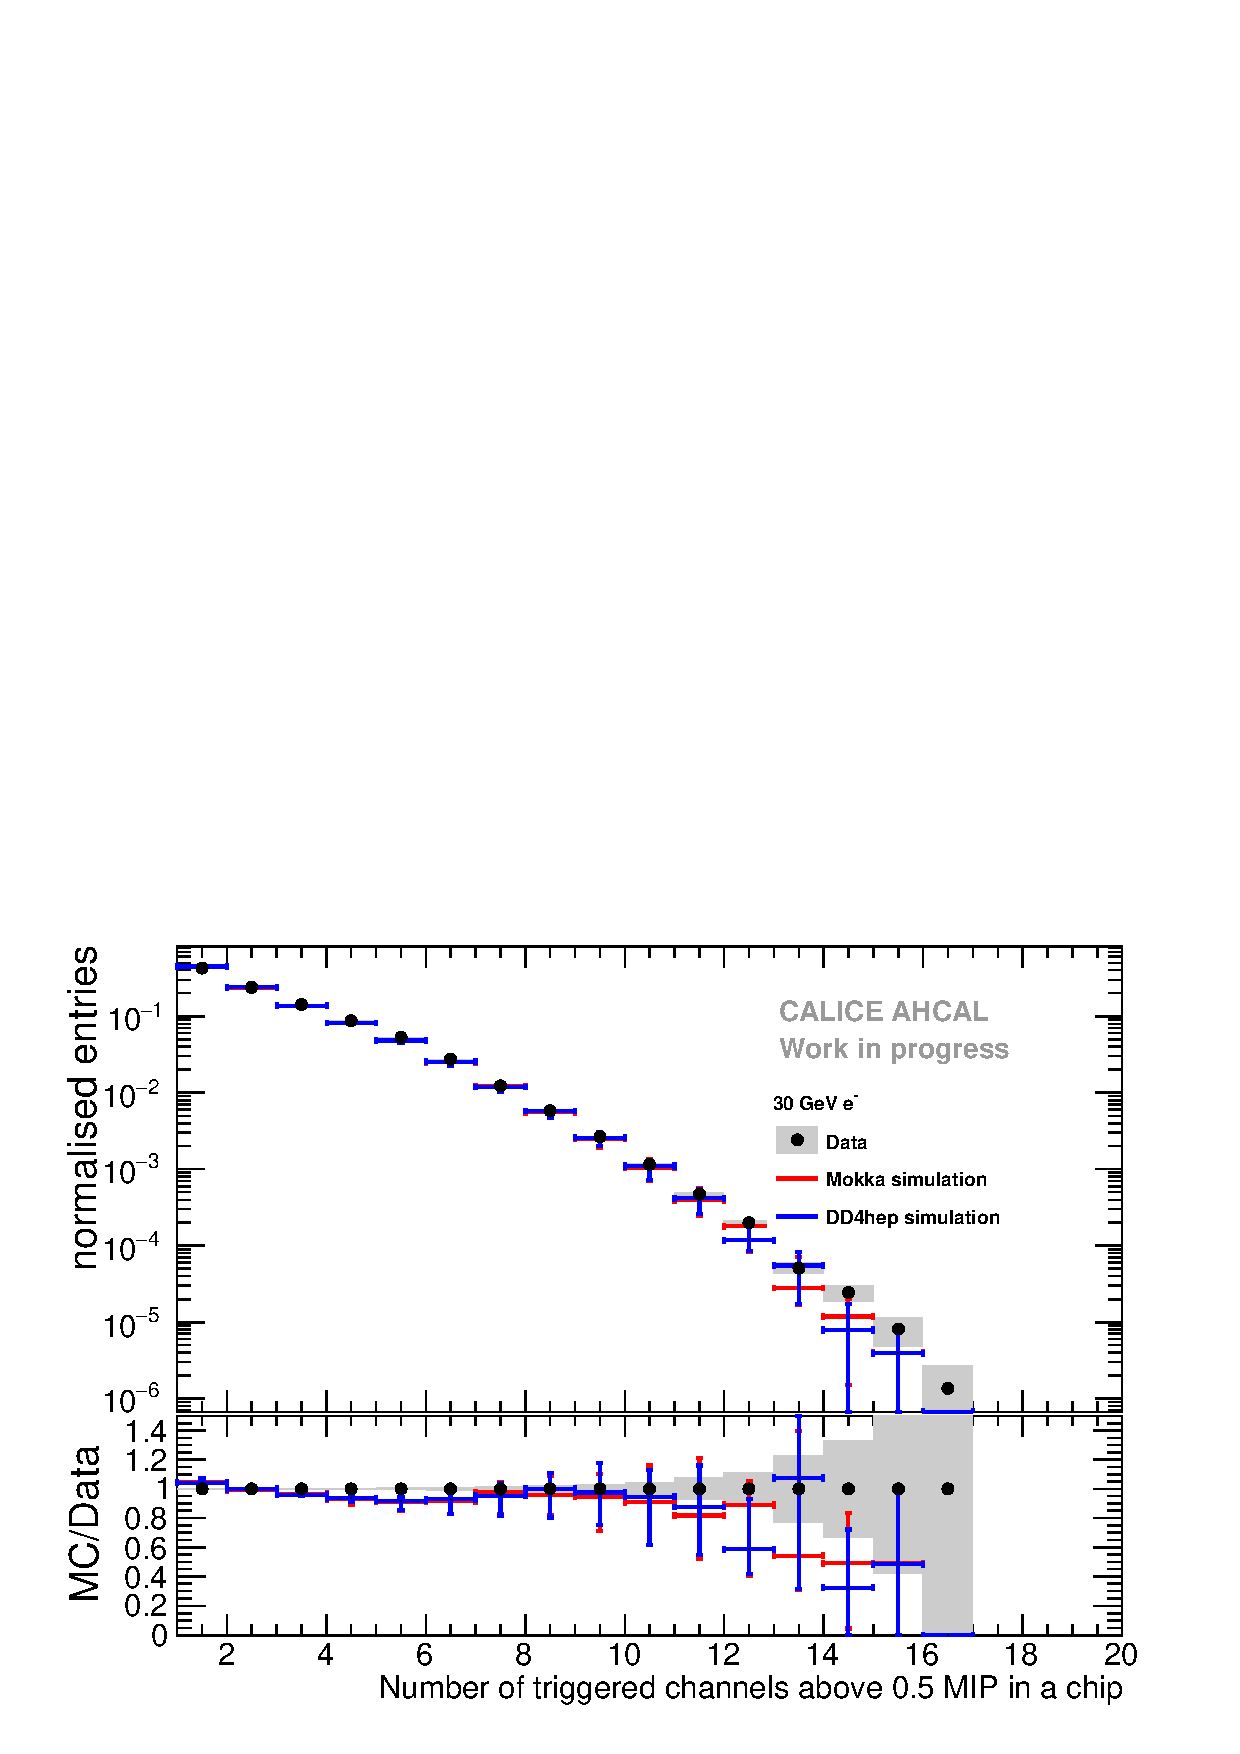
\includegraphics[width=1\textwidth]{../Thesis_Plots/Timing/Electrons/Plots/Comparison_SimData_Electrons_nHits_30GeV.pdf}
    \caption{30 GeV.}\label{fig:elec_sim_data_nHits_30GeV}
  \end{subfigure}
  \hfill
  \begin{subfigure}[t]{0.5\textwidth}
    \centering
    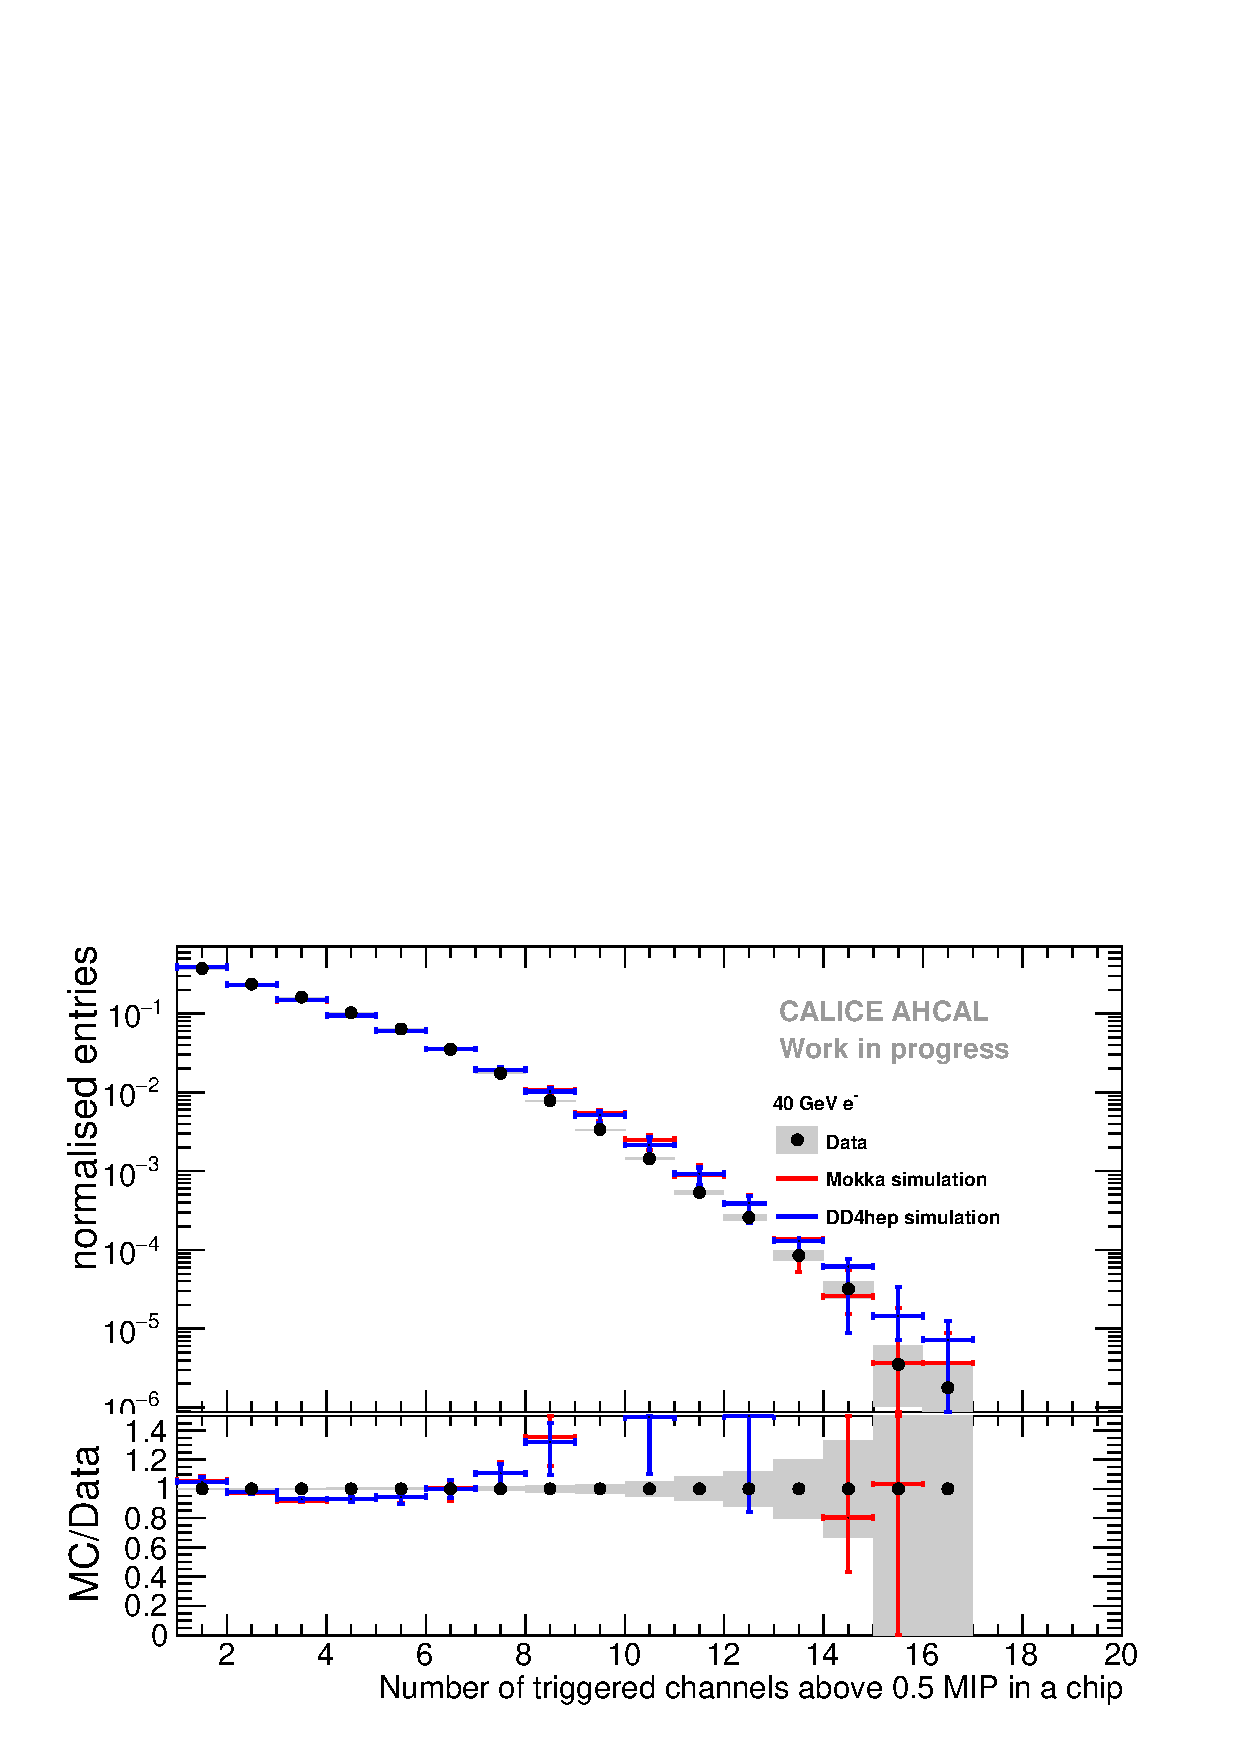
\includegraphics[width=1\textwidth]{../Thesis_Plots/Timing/Electrons/Plots/Comparison_SimData_Electrons_nHits_40GeV.pdf}
    \caption{40 GeV.}\label{fig:elec_sim_data_nHits_40GeV}
  \end{subfigure}
  \hfill
  \begin{subfigure}[t]{0.5\textwidth}
    \centering
    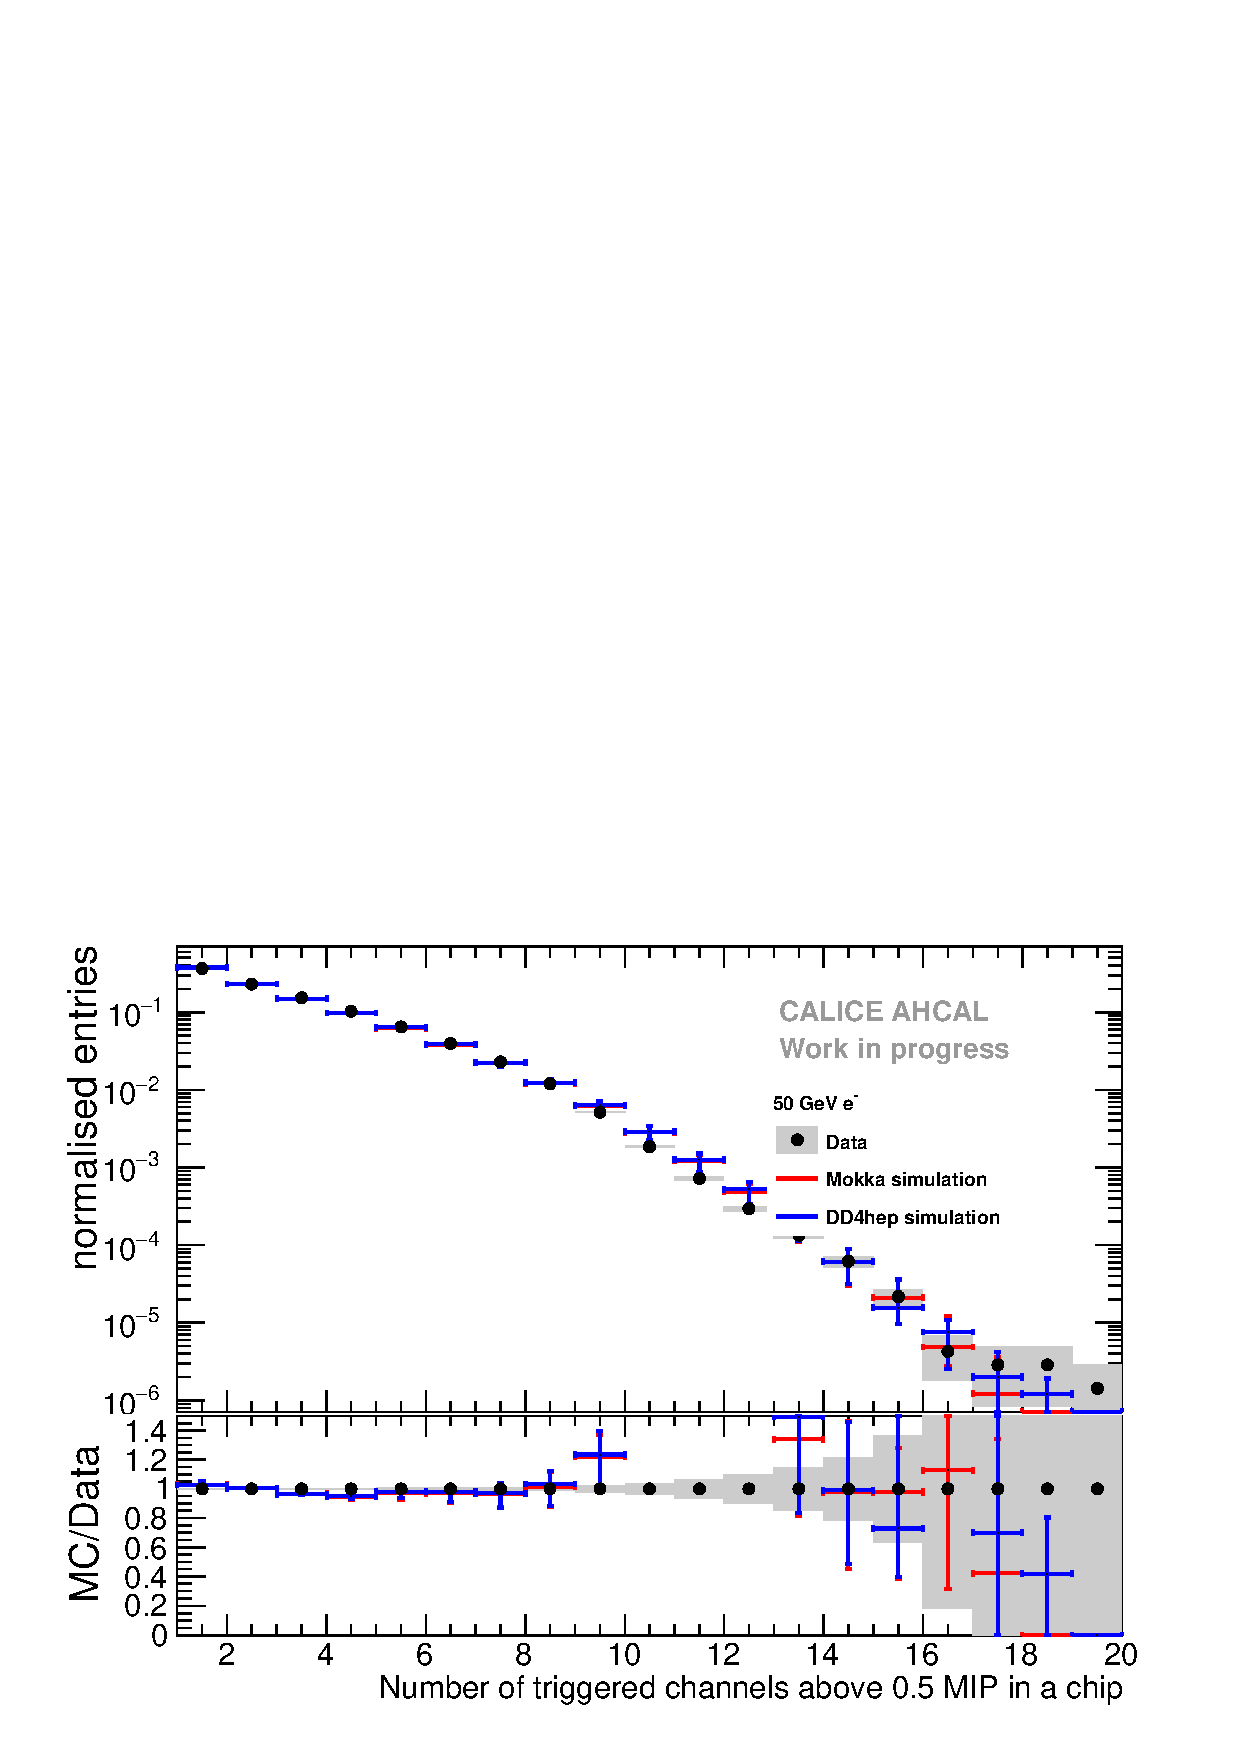
\includegraphics[width=1\textwidth]{../Thesis_Plots/Timing/Electrons/Plots/Comparison_SimData_Electrons_nHits_50GeV.pdf}
    \caption{50 GeV.}\label{fig:elec_sim_data_nHits_50GeV}
  \end{subfigure}
  \caption{Comparison between electron data and MC for all energies of the number of triggered channels per chip. The grey area represents the statistical error of the data. Error bars in simulation are obtained by varying the cross-talk parameter between 10\% and 18\%.}
  \label{fig:sim_data_elec_nHits}
\end{figure}
